\documentclass[10pt]{article}
\usepackage[margin=1in]{geometry}
\usepackage{amsmath,amssymb,amsthm}
\usepackage{graphicx}
\usepackage{booktabs}
\usepackage{hyperref}
\usepackage{xcolor}
\usepackage[numbers,sort&compress]{natbib}
\usepackage{subcaption}
\usepackage{multirow}
\usepackage{longtable}
\usepackage{lineno}
\usepackage{setspace}
\graphicspath{{figures/}}

\newtheorem{proposition}{Proposition}
\newtheorem{corollary}[proposition]{Corollary}

\newcommand{\citeneeded}[1]{\textcolor{red}{[CITE: #1]}}
\newcommand{\todo}[1]{\textcolor{orange}{[TODO: #1]}}

\title{Most knockout epistasis is generated by dynamics, not molecular wiring}

\author{
  Elliot Tower\textsuperscript{1,*} \\[4pt]
  \small\textsuperscript{1}Independent Researcher \\
  \small\textsuperscript{*}Correspondence: \texttt{elliot@elliottower.ai}
}

\begin{document}
\maketitle
\linenumbers
\doublespacing

\begin{abstract}
Nonlinear dynamics generate phenotypic epistasis from molecular
architectures that may contain no epistatic interactions themselves.
Prior work established this gap qualitatively; we quantify it
order-by-order across 27 published Boolean gene regulatory networks
(7--17 genes). For each network, we compute the complete
Walsh--Hadamard interaction spectrum at two levels: the local update
rules and the attractor-level knockout landscape from exhaustive
$2^n$ coalition sweeps. Comparing the two spectra reveals a signed
\emph{composition gap} spanning three orders of magnitude ($< 1$ to
$+83$ percentage points of order-3+ energy). Creation of higher-order
interactions is the dominant mode: 18 of 24 non-null networks show
positive gaps, with a median of $+8.5$~pp. Pairwise Spearman
correlation between local and global interaction magnitudes is positive
on average (median $\rho = 0.27$, significant in 16/27 networks) but
negative in five, demonstrating that molecular wiring is a noisy and
sometimes misleading predictor of knockout epistasis. Limit-cycle prevalence correlates negatively with the composition gap
(discovered on 6 networks, same direction on 21 held-out networks:
$\rho = -0.37$, $p = 0.10$), though counterexamples in both
directions preclude a clean threshold. Pre-registered structural
predictions on 21 held-out networks---including a feedback loop ratio
hypothesis---perform at chance on gap direction (10/21, 48\%),
establishing that the composition gap is not reducible to simple
topological features of the regulatory graph. The same Walsh
decomposition applied to three experimental fitness landscapes---the
Weinreich TEM-1 beta-lactamase (5 mutations, 32 genotypes), Hall
yeast biosynthetic knockouts (6 genes, 64 genotypes), and the
Franke \emph{Aspergillus niger} sporulation landscape (8 loci,
256 genotypes)---confirms that higher-order epistasis exceeding
pairwise structural or pathway predictions is present in real
organisms, with magnitude depending on the fitness component
measured. Converting 20 networks (of 27) to
Hill-function ODEs preserves the sign of the gap in all 20 cases,
confirming that the effect is a property of
regulatory topology rather than Boolean discretization. The complete Walsh spectra, coalition value functions, and
pre-registration artifacts are released for reuse.
\end{abstract}

\noindent\textbf{Keywords:}
epistasis, Boolean networks, gene regulatory networks,
Walsh--Hadamard transform, composition gap, knockout screens


\section*{Author summary}
Genes rarely act alone: knocking out multiple genes often produces
effects that no single knockout predicts. Biologists call this epistasis.
The molecular wiring of a gene regulatory network specifies pairwise
interactions, but the phenotype depends on the long-run dynamics of the
entire network. We ask: does dynamical composition systematically create
or destroy higher-order epistasis? Across 27 published Boolean network
models, we find that dynamics create higher-order interactions three
times more often than they destroy them. The molecular wiring diagram
provides some guidance---local interaction strength correlates with
knockout epistasis in most networks---but it fails as a reliable
predictor: five networks show reversed correlations, and structural
features predict the sign of the gap at chance. These results mean
that knockout screens probe an epistatic landscape shaped as much by
dynamics as by molecular mechanism. Analysis of three experimental
fitness landscapes---a protein resistance landscape, yeast
biosynthetic knockouts, and a fungal sporulation landscape---confirms
that higher-order epistasis exceeding pairwise structural predictions
is present in real organisms.


%% ====================================================================
\section{Introduction}
\label{sec:intro}
%% ====================================================================

Epistasis---the dependence of phenotype on gene combinations rather
than individual effects---is among the oldest measurement problems in
quantitative genetics \citep{fisher1918correlation, bateson1909heredity}. A
persistent difficulty is the gap between molecular and statistical
epistasis: the interactions encoded in regulatory logic need not
predict the interactions observed in knockout experiments
\citep{phillips2008epistasis}. \citet{gjuvsland2007statistical} showed
that nonlinear dynamics generically produce statistical epistasis from
gene regulatory architectures, regardless of whether the underlying
molecular rules contain epistatic terms. Subsequent work confirmed this in synthetic three-gene
circuits, where pairwise and triplet epistasis depended on environment
and switched sign across conditions \citep{baier2023environment}.

These results establish that a gap exists. They do not quantify it.
The gap has no known magnitude, no known sign structure, and no
established dependence on network architecture. One reason is
computational: exhaustive knockout measurement requires $2^n$ subset
evaluations, which is infeasible at genomic scale. In Boolean gene
regulatory networks of modest size ($n \leq 17$), however, exhaustive
evaluation is tractable.

We exploit this tractability across 27 published Boolean networks
spanning cell-cycle control, apoptosis, differentiation, DNA repair,
and developmental patterning. For each network, we compute two
complete interaction spectra using the Walsh--Hadamard transform: one
from the local update rules and one from the attractor-level value
function. The two spectra are compared order-by-order, yielding a
signed composition gap that measures how much higher-order structure
dynamics create or destroy.

Three findings emerge. First, creation is the dominant mode: dynamics
more often generate higher-order interactions than destroy them (18/24
non-null networks). Second, the molecular wiring diagram is a noisy
and sometimes misleading predictor of knockout epistasis---positive on
average but negative in five networks. Third, pre-registered
structural predictions perform at chance on gap direction (48\%),
establishing that the composition gap is not reducible to network
topology.


%% ====================================================================
\section{Methods}
\label{sec:methods}
%% ====================================================================

\subsection{Boolean network models}
\label{sec:models}

Twenty-seven published Boolean gene regulatory networks were collected
from the Cell Collective repository \citep{helikar2012cell}, the
PyBoolNet model repository \citep{klarner2017pyboolnet}, the Biodivine
Boolean Models repository, and primary literature. Selection criteria:
(i)~$n \leq 18$ nodes to permit exhaustive $2^n$ coalition sweeps
within a day of CPU time, (ii)~synchronous update semantics used or
compatible with the original publication, and (iii)~a biologically
interpretable output node. The networks span cell-cycle control
(mammalian, yeast, \emph{Drosophila}, \emph{Arabidopsis}), apoptosis,
hematopoietic differentiation, DNA repair, developmental patterning,
gene regulation, and signal transduction (Table~\ref{tab:all_results}).

To guard against overfitting structural hypotheses to results, the
models were analyzed in two batches. Batch~1 (6~networks) was used to
develop the analysis pipeline and formulate structural predictions.
Batch~2 (21~networks) was analyzed blind: structural predictions were
SHA-frozen before any coalition sweep ran
(Section~\ref{sec:blind}).


\subsection{Local rule Fourier extraction}
\label{sec:local-fourier}

Each gene $k$ has a Boolean update rule $f_k\colon \{0,1\}^{r_k}
\to \{0,1\}$, where $r_k$ is the number of regulators. We compute
the Walsh--Hadamard transform of the truth table:
%
\begin{equation}
\label{eq:local-wht}
w_T^{(k)} = \frac{1}{2^{r_k}} \sum_{x \in \{0,1\}^{r_k}} f_k(x)\,(-1)^{|x \cap T|},
\quad T \subseteq \{1, \ldots, r_k\}.
\end{equation}
%
A nonzero coefficient $w_T^{(k)}$ at $|T| = m$ indicates a genuine
$m$-way interaction among the regulators of gene $k$,
representation-independent. For each unordered pair $\{i,j\}$ of
network genes, the \emph{local pairwise magnitude} is:
%
\begin{equation}
\label{eq:local-pair}
\ell_{ij} = \sum_{k:\, i,j \in \mathrm{reg}(k)} |w_{\{i,j\}}^{(k)}|,
\end{equation}
%
summing over all genes $k$ whose update rule depends on both $i$ and
$j$. The \emph{local energy spectrum} reports the fraction of total
squared-coefficient energy at each interaction order~$m$:
%
\begin{equation}
\label{eq:local-spectrum}
E_m^{\mathrm{local}} = \frac{\sum_k \sum_{|T|=m} \bigl(w_T^{(k)}\bigr)^2}
{\sum_k \sum_T \bigl(w_T^{(k)}\bigr)^2}.
\end{equation}


\subsection{Coalition sweep and attractor-level value function}
\label{sec:coalition-sweep}

For each of $2^n$ coalitions $S \subseteq \{1,\ldots,n\}$, genes not
in $S$ are clamped to~0 (knockout). The remaining genes evolve under
synchronous Boolean dynamics from $N = 512$ uniformly random initial
states until convergence to a fixed point or limit cycle (detected by
Floyd's algorithm, maximum 200 steps). The value function is:
%
\begin{equation}
\label{eq:value}
v(S) = \frac{1}{N} \sum_{i=1}^{N}
\overline{x_{\mathrm{out}}^{(i)}(S)},
\end{equation}
%
where $\overline{x_{\mathrm{out}}^{(i)}(S)}$ is the time-averaged
output-node state for initial condition $i$ under coalition $S$. The
global Walsh--Hadamard transform of $v$ gives the \emph{global
interaction spectrum}:
%
\begin{equation}
\label{eq:global-wht}
w_T^{\mathrm{global}} = \frac{1}{2^n} \sum_{S \subseteq \{1,\ldots,n\}}
v(S)\,(-1)^{|S \cap T|}.
\end{equation}
%
The global pairwise magnitude is
$g_{ij} = |w_{\{i,j\}}^{\mathrm{global}}|$, and the
\emph{global energy spectrum} is defined analogously to
Eq.~\ref{eq:local-spectrum}.


\subsection{Composition gap metrics}
\label{sec:metrics}

\textbf{Pairwise Spearman correlation.}
For each network, $\rho = \mathrm{Spearman}(\ell_{ij}, g_{ij})$ over
all $\binom{n}{2}$ pairs, with bootstrap 95\% CIs (10{,}000
resamples).

\textbf{Order-3+ energy gap.}
$\Delta_{3+} = \sum_{m \geq 3} E_m^{\mathrm{global}}
- \sum_{m \geq 3} E_m^{\mathrm{local}}.$
Positive $\Delta_{3+}$ indicates creation; negative indicates
destruction. Networks with $|\Delta_{3+}| < 0.5$~pp are classified as
null.

\textbf{Quality gate.}
The global spectrum is analyzed only if (i)~the value function has
$\geq 10$ unique values, (ii)~absolute order-3+ energy exceeds
$10^{-4}$, and (iii)~no single value accounts for $> 90\%$ of
coalitions. All 27~networks pass.


\subsection{Blind prediction protocol}
\label{sec:blind}

Structural predictions were registered in two batches before coalition
sweeps ran. For Batch~1 (6~networks), predictions were based on
Boolean rule analysis, feedback loop topology, and output-node
structure. A cross-network hypothesis was registered: positive
feedback loop ratio $> 0.5$ implies creation. For Batch~2
(21~networks), predictions used the same structural analysis applied
independently. All predictions were SHA-frozen before any sweep
executed.


%% ====================================================================
\subsection{Theoretical framework: algebraic and dynamical composition}
\label{sec:theory}

The composition gap admits a natural decomposition into two
mechanistically distinct components. We formalize each with a
proposition and derive an empirically testable prediction.

\begin{proposition}[Acyclic convergence]
\label{prop:dag}
Let $G$ be a Boolean network whose regulatory graph $\Gamma$ is
acyclic (after removing identity-function input nodes). Then for every
knockout set $S$ and every initial condition, synchronous dynamics
converge to a fixed point within $\mathrm{depth}(\Gamma)$ steps.
The fixed point is unique for each input-node configuration.
\end{proposition}

\begin{proof}
Label the non-input nodes $1, \ldots, m$ in topological order. At
step $t$, node~$i$'s update depends only on nodes with indices
$< i$. After one complete pass through the topological order, all
source nodes have reached their steady values; after two passes, all
nodes at depth~2 have stabilized; and so on. After
$d = \mathrm{depth}(\Gamma)$ steps, every node's value is
self-consistent, and the state repeats thereafter. Because each
node's steady value is a deterministic function of the source
(input-node) values and the clamping configuration, the fixed point
is unique given the input configuration.
\end{proof}

Proposition~\ref{prop:dag} establishes that acyclic networks have no
dynamical degrees of freedom: no limit cycles, no basin-dependent
output variation. The value function $v(S)$ reduces to the composed
Boolean function evaluated at a single (or input-averaged) fixed
point. Any composition gap in a DAG arises from algebraic composition
of local rules along regulatory paths, not from attractor dynamics.

\begin{proposition}[Algebraic creation of higher-order epistasis]
\label{prop:creation}
There exist acyclic Boolean networks in which every local rule has
Walsh order $\leq 2$, yet the composed value function has nonzero
Walsh coefficients at order~3 or higher.
\end{proposition}

\begin{proof}
Consider four genes $x_1, x_2, x_3, y$ with rules
$h = x_1 \wedge x_2$ and $y = h \wedge x_3$, arranged as a
depth-2 DAG. Each local rule has two regulators and Walsh order~2.
The composed function $y(S) = (x_1 \wedge x_2) \wedge x_3$ has
Walsh expansion (in $\pm 1$ encoding)
$y = \tfrac{1}{8}(1 - z_1 - z_2 - z_3 + z_1 z_2 + z_1 z_3
+ z_2 z_3 - z_1 z_2 z_3)$,
where $z_i = 1 - 2x_i$. The $z_1 z_2 z_3$ term has order~3,
so the global Walsh spectrum contains energy at order~3 that is
absent from every local rule's spectrum.
\end{proof}

More generally, iterated composition through a depth-$d$ path can
raise the Walsh order to $\min(n,\, d \cdot k)$, where $k$ is the
maximum local Walsh order. This algebraic mechanism suffices to
explain creation even in the absence of feedback.

For networks with feedback, a second mechanism emerges. Feedback
loops create multiple attractors (fixed points and limit cycles)
whose basins partition the state space. Different knockout sets
reroute initial conditions across basin boundaries, introducing
sharp coalition-dependent transitions that encode higher-order
interactions. Simultaneously, limit cycles introduce a competing
effect: time-averaging the output node over a cycle period acts as
a low-pass filter on the value function, compressing higher-order
Walsh coefficients.

\begin{corollary}[Decomposition of the composition gap]
\label{cor:decomposition}
The composition gap decomposes as
$\Delta_{3+} = \Delta_{\mathrm{alg}} + \Delta_{\mathrm{dyn}}$,
where $\Delta_{\mathrm{alg}}$ arises from path-wise composition of
local rules (present in all networks, including DAGs) and
$\Delta_{\mathrm{dyn}}$ arises from attractor basin geometry
(zero in DAGs, nonzero in networks with feedback). The sign and
magnitude of $\Delta_{\mathrm{dyn}}$ depend on whether
basin-boundary effects (which amplify higher-order structure) or
cycle-averaging effects (which attenuate it) dominate.
\end{corollary}

This decomposition predicts that cycling fraction---the proportion
of (coalition, initial state) pairs entering limit cycles---should
correlate negatively with $\Delta_{3+}$ if cycle-averaging
dominates, and positively if basin-boundary effects dominate.
Section~\ref{sec:cycling} tests this prediction empirically.


\subsection{Hill-function ODE conversion}
\label{sec:ode-method}

The Boolean discretization is a modeling choice, not a biological
fact. To test whether the composition gap survives under continuous
dynamics, we convert Boolean rules to Hill-function ODEs. Each node
$i$ evolves as
\begin{equation}
  \frac{dx_i}{dt} = \frac{1}{\tau}
  \left( \sigma\!\left(f_i^{\mathrm{cont}}(\mathbf{x})\right) - x_i \right),
\end{equation}
where $f_i^{\mathrm{cont}}$ replaces Boolean operators with smooth
approximations (AND $\to$ product, OR $\to$ probabilistic OR
$a + b - ab$, NOT $\to$ $1 - x$) and $\sigma(z) = z^{n_H} / (z^{n_H} + K^{n_H})$
is a Hill sigmoid with cooperativity $n_H = 10$ and half-max $K = 0.5$.
Knocked-out genes are clamped to zero via a stiff restoring term.

For each coalition, the ODE system is integrated from 32 random
initial conditions using RK45 (SciPy \texttt{solve\_ivp},
$t_{\max} = 30$, rtol $= 10^{-4}$). The output is time-averaged
over the final third of the trajectory to capture limit-cycle
behavior. The coalition value function and Walsh decomposition
proceed identically to the Boolean analysis.

The local Walsh spectrum is identical under Boolean and ODE dynamics
because the local rules do not change; only the global dynamics
differ. The ODE composition gap is therefore
$\Delta_{3+}^{\mathrm{ODE}} = E_{3+}^{\mathrm{ODE,global}} - E_{3+}^{\mathrm{local}}$.


\subsection{Empirical fitness landscape analysis}
\label{sec:empirical-method}

To test whether the composition gap generalizes beyond simulation,
we apply the Walsh decomposition to two published combinatorial
fitness datasets where the full $2^n$ landscape is measured
experimentally.

\paragraph{Weinreich TEM-1 beta-lactamase.}
\citet{weinreich2006darwinian} measured cefotaxime minimum
inhibitory concentration (MIC) for all 32 genotypes formed by 5
binary mutations in TEM-1 beta-lactamase. MIC values span a
$\sim$47{,}000-fold range (0.071--4100~$\mu$g/mL), so we analyze
log-transformed values. The local interaction structure is defined
by structural contacts from the crystal structure (PDB 1BTL): two
mutation sites interact locally if their C$\alpha$--C$\alpha$
distance is $\leq 8$~\AA. No pairs meet this threshold (closest:
E104K--G238S at 12.67~\AA), so the local model is purely additive
and $E_{3+}^{\mathrm{local}} = 0$.

\paragraph{Hall yeast biosynthetic knockouts.}
\citet{hall2010fitness} measured four fitness components (haploid
growth rate, diploid growth rate, mating efficiency, sporulation
efficiency) for all 64 genotypes formed by 6 biosynthetic gene
knockouts in \emph{S.~cerevisiae}. Each gene catalyzes a step in a
distinct biosynthetic pathway (amino acids, nucleotides, or
vitamins). The pathways share upstream precursors from central
carbon metabolism (PRPP, TCA cycle intermediates), but the exact
locus-to-gene mapping is unavailable from the public data, so the
local model is conservatively set to additive
($E_{3+}^{\mathrm{local}} = 0$). All four fitness components are
analyzed; haploid growth rate is the primary measure.

\paragraph{Franke \emph{Aspergillus niger} sporulation.}
\citet{franke2011evolutionary} measured sporulation efficiency for
186 of 256 genotypes formed by 8 binary loci in
\emph{Aspergillus niger}. Seventy genotypes showed no measurable
sporulation (lethal or near-lethal). We analyze the full 186-genotype
dataset both with and without these zero-fitness genotypes, since
lethality may inflate apparent higher-order interactions through
floor effects. The local model is additive
($E_{3+}^{\mathrm{local}} = 0$), as the loci span distinct
biosynthetic and developmental pathways.

For all three datasets, the composition gap equals the global order-3+
energy fraction, measuring how much higher-order epistasis exists
in the fitness landscape beyond what a purely additive local model
predicts.


%% ====================================================================
\section{Results}
\label{sec:results}
%% ====================================================================

\subsection{Creation is the dominant mode}

Table~\ref{tab:all_results} summarizes all 27 networks. Of 24
non-null networks ($|\Delta_{3+}| \geq 0.5$~pp), 18 show creation
and 6 show destruction. The median $\Delta_{3+}$ is $+8.5$~pp, and
the mean is $+20$~pp. The gap magnitudes span three orders: from
effectively zero (Davidich yeast, $-0.4$~pp; Remy p53, $+0.08$~pp)
to $+83$~pp (cell-cycle transcription network). This creation bias
indicates that nonlinear dynamics more often generate higher-order
epistasis than compress it (Figure~\ref{fig:delta-ranked}).

\begin{figure}[t]
\centering
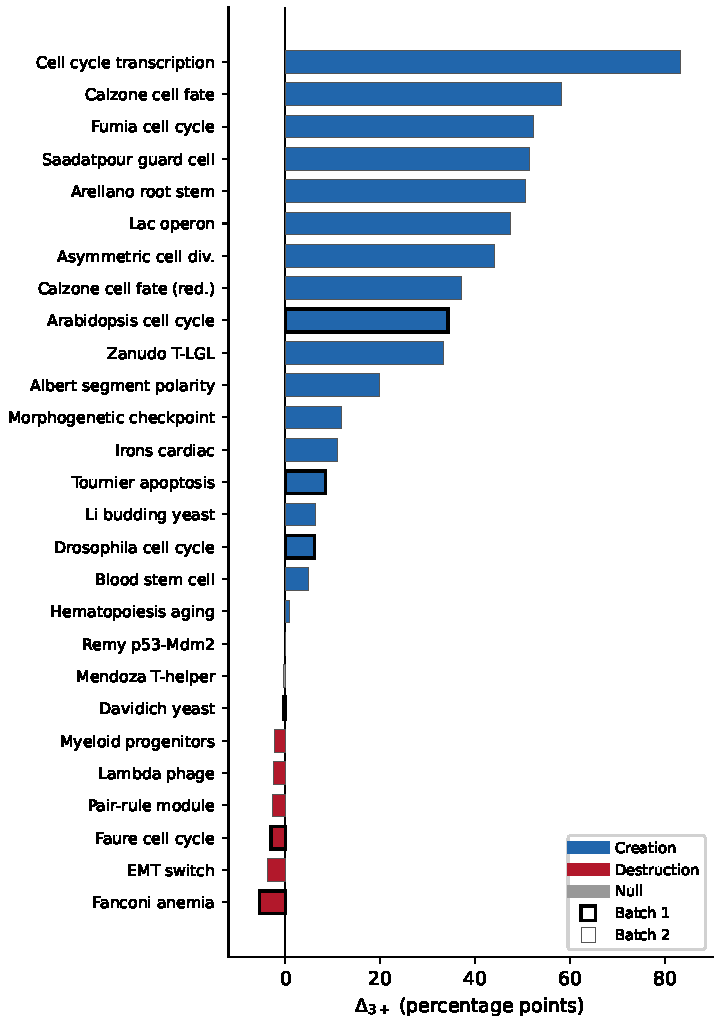
\includegraphics[width=0.65\textwidth]{fig1_delta_ranked.pdf}
\caption{Composition gap ($\Delta_{3+}$) for all 27 networks, ranked
by magnitude. Blue: creation (positive gap). Red: destruction
(negative gap). Gray: null ($|\Delta_{3+}| < 0.5$~pp). Thick
borders indicate batch~1 networks; thin borders indicate batch~2
(held-out). The gap spans three orders of magnitude, from
effectively zero to $+83$~pp.}
\label{fig:delta-ranked}
\end{figure}

\begin{longtable}{lrrrrl}
\caption{Composition gap results for 27 Boolean GRNs, sorted by
cycling fraction. $\rho$: Spearman correlation between local and
global pairwise magnitudes. $\Delta_{3+}$: global minus local
order-3+ energy (pp). Classification: creation ($> 0.5$~pp),
destruction ($< -0.5$~pp), or null.}
\label{tab:all_results} \\
\toprule
Network & $n$ & $\rho$ & $p$ & $\Delta_{3+}$ & Cycling \\
\midrule
\endfirsthead
\toprule
Network & $n$ & $\rho$ & $p$ & $\Delta_{3+}$ & Cycling \\
\midrule
\endhead
\bottomrule
\endfoot
Arellano root stem & 9 & 0.60 & $< 10^{-4}$ & $+$50.6 & 0.0\% \\
Segment polarity & 11 & 0.21 & 0.126 & $+$19.8 & 0.0\% \\
EMT switch & 12 & 0.38 & 0.002 & $-$3.8 & 0.1\% \\
Lac operon & 13 & 0.08 & 0.492 & $+$47.4 & 0.3\% \\
Cell cycle transcription & 9 & $-$0.38 & 0.021 & $+$83.3 & 0.4\% \\
Morphogenetic checkpoint & 12 & 0.40 & $< 10^{-3}$ & $+$11.9 & 0.4\% \\
Calzone cell fate (full) & 17 & $-$0.02 & 0.855 & $+$58.2 & 0.5\% \\
Mendoza T-helper$^\dagger$ & 13 & 0.21 & 0.059 & $-$0.3 & 1.7\% \\
Saadatpour guard cell & 13 & 0.07 & 0.572 & $+$51.4 & 5.7\% \\
Asymmetric cell division & 9 & $-$0.10 & 0.547 & $+$44.1 & 6.3\% \\
Myeloid progenitors & 11 & 0.51 & $< 10^{-4}$ & $-$2.3 & 6.6\% \\
Tournier apoptosis & 12 & 0.25 & 0.046 & $+$8.5 & 7.4\% \\
Irons cardiac & 15 & 0.63 & $< 10^{-12}$ & $+$10.9 & 9.3\% \\
Za\~nudo T-LGL & 12 & $-$0.19 & 0.120 & $+$33.2 & 10.3\% \\
Hematopoiesis aging & 15 & 0.63 & $< 10^{-12}$ & $+$0.9 & 10.5\% \\
Calzone cell fate (reduced) & 11 & $-$0.07 & 0.586 & $+$37.0 & 11.1\% \\
Li budding yeast & 11 & 0.53 & $< 10^{-4}$ & $+$6.3 & 12.5\% \\
Fumia cell cycle & 14 & 0.27 & 0.011 & $+$52.2 & 12.5\% \\
Remy p53-Mdm2$^\dagger$ & 10 & 0.50 & $< 10^{-3}$ & $+$0.1 & 13.4\% \\
\emph{Drosophila} cell cycle & 14 & 0.12 & 0.257 & $+$6.2 & 14.0\% \\
Lambda phage & 7 & 0.61 & 0.004 & $-$2.5 & 16.0\% \\
\emph{Arabidopsis} cell cycle & 14 & 0.21 & 0.052 & $+$34.3 & 16.4\% \\
Davidich yeast$^\dagger$ & 10 & 0.15 & 0.312 & $-$0.4 & 17.7\% \\
Pair-rule module & 11 & 0.66 & $< 10^{-7}$ & $-$2.7 & 17.8\% \\
Faure cell cycle & 10 & 0.41 & 0.005 & $-$3.0 & 19.6\% \\
Blood stem cell & 11 & 0.59 & $< 10^{-5}$ & $+$4.8 & 24.5\% \\
Fanconi anemia & 15 & 0.31 & 0.002 & $-$5.5 & 47.5\% \\
\midrule
\multicolumn{6}{l}{\footnotesize $^\dagger$Null: $|\Delta_{3+}| < 0.5$~pp.} \\
\multicolumn{6}{l}{\footnotesize 18 creation, 6 destruction, 3 null out of 27 networks.} \\
\end{longtable}


\begin{figure}[t]
\centering
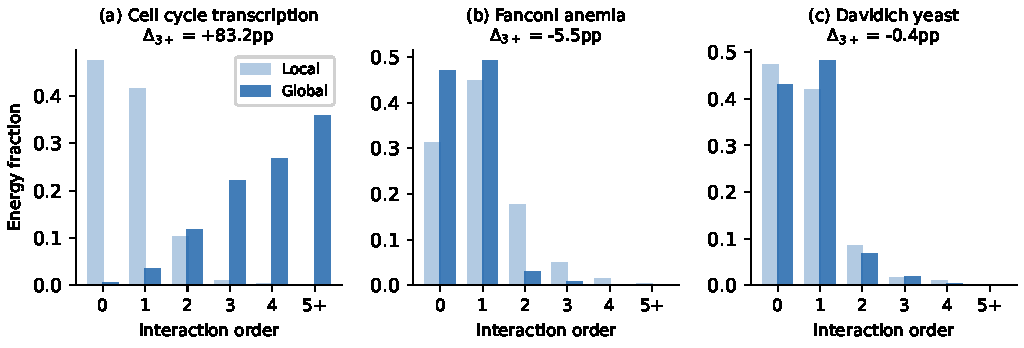
\includegraphics[width=\textwidth]{fig3_spectrum_comparison.pdf}
\caption{Local (hatched) and global (solid) energy spectra for three
representative networks. (a)~Cell-cycle transcription
($\Delta_{3+} = +83$~pp): local rules concentrate energy at orders
0--2; dynamics redistribute it into orders 3+. (b)~Fanconi anemia
($\Delta_{3+} = -5.5$~pp): dynamics compress higher-order structure.
(c)~Davidich yeast ($\Delta_{3+} = -0.4$~pp): near-identical spectra
(null case).}
\label{fig:spectrum}
\end{figure}

\subsection{Local--global correlation is positive on average but not universal}
\label{sec:rho}

The median Spearman $\rho$ between local and global pairwise
magnitudes is $0.27$ (mean $0.28$). Sixteen of 27 networks have
significant positive correlations ($p < 0.05$). In these networks,
the molecular wiring diagram provides a useful prior for predicting
which gene pairs will show knockout epistasis.

Five networks show negative $\rho$, and one of these
(cell-cycle transcription, $\rho = -0.38$, $p = 0.02$) is
statistically significant. In this network, gene pairs with strong
local Fourier interactions tend to have \emph{weaker} global knockout
epistasis. Negative correlations indicate that dynamical composition
can actively invert the interaction structure encoded in local rules.

The remaining six networks have non-significant positive
correlations, where the molecular wiring diagram carries no detectable
information about knockout epistasis.


\subsection{Limit-cycle prevalence correlates with the composition gap}
\label{sec:cycling}

The theoretical decomposition (Corollary~\ref{cor:decomposition})
predicts that cycling fraction should correlate with $\Delta_{3+}$,
with the sign depending on whether cycle-averaging or basin-boundary
effects dominate. A negative association between cycling fraction and $\Delta_{3+}$ was
observed post-hoc on the 6 batch-1 networks ($\rho = -0.83$,
$p = 0.04$, but post-hoc so effectively $\sim 0.10$ two-tailed),
consistent with cycle-averaging dominance.
This pattern was then tested on the 21 held-out batch-2 networks:
the correlation has the same sign but is not independently
significant ($\rho = -0.37$, $p = 0.10$, $N = 21$). Pooling all 27
networks gives $\rho = -0.51$ ($p = 0.007$), but this combined
statistic includes the discovery sample and should be interpreted
accordingly.

Among non-null networks, the destruction group has a higher median
cycling fraction (16.9\%) than the creation group (8.3\%), but the
distributions overlap substantially and a Mann--Whitney test on the
categorical split is not significant ($U = 30$, $p = 0.12$). The
continuous correlation does not corroborate a clean categorical
separation: counterexamples exist in both directions. EMT switch has
$0.1\%$ cycling but shows destruction ($-3.8$~pp), and blood stem
cell has $24.5\%$ cycling but shows creation ($+4.8$~pp).

This direction is consistent with the cycle-averaging mechanism
described in Section~\ref{sec:theory}: time-averaging output over
limit-cycle periods smooths coalition-dependent variation in attractor
structure, compressing higher-order Walsh coefficients. Fixed-point
attractors preserve discrete switching behavior, allowing
combinatorial interactions to compound. Cycling fraction does not
correlate with network size ($\rho = 0.09$, $p = 0.87$, $N = 27$),
so this association is not a proxy for the number of genes. The
cycling hypothesis remains suggestive and awaits confirmation on an
independent sample.


\subsection{Structural predictions perform at chance}
\label{sec:blind-results}

The confirmatory test of structural predictions is batch~2, where
predictions were made on 21 networks whose composition gaps had not
been computed. Direction accuracy on batch~2 was 10/21 (48\%),
indistinguishable from chance (Table~\ref{tab:blind}). Predicted
$\rho$ ranges contained the observed value in 6/21 cases (29\%). A
pre-registered cross-network hypothesis (positive feedback loop ratio
$> 0.5$ implies creation) was falsified in both batches.

Batch~1 predictions (4/6 direction accuracy) were developed on the
same 6 networks they are scored against and are therefore circular;
they are reported for completeness but are not evidence of predictive
power.

\begin{table}[t]
\centering
\caption{Blind prediction accuracy. Batch~2 (21 held-out networks) is
the confirmatory test; batch~1 predictions were developed on the same
networks and are circular. Predictions were SHA-frozen before
coalition sweeps ran.}
\label{tab:blind}
\begin{tabular}{lccc}
\toprule
Category & Batch 2 (confirmatory) & Batch 1 (circular) \\
\midrule
Gap direction & 10/21 (48\%) & 4/6 \\
$\rho$ in predicted range & 6/21 (29\%) & 4/6 \\
fb\_ratio hypothesis & Falsified & Falsified \\
\bottomrule
\end{tabular}
\end{table}

This result is itself informative. The composition gap is not
predictable from the structural features most commonly used to
characterize Boolean networks: feedback loop counts, rule complexity,
in-degree distribution, and output-node arity. Predicting whether
dynamics will create or destroy higher-order epistasis requires
information about the full composed dynamical system that cannot be
extracted from local rules or network topology alone.


\subsection{The composition gap survives continuous dynamics}
\label{sec:ode-results}

To test whether the composition gap is an artifact of Boolean
discretization, we converted 20 of 27 networks ($n = 7$--15) to
Hill-function ODEs (Section~\ref{sec:ode-method}) and recomputed
the coalition sweep under continuous dynamics.
Table~\ref{tab:ode} summarizes the results.

\begin{table}[t]
\centering
\caption{Composition gap under Boolean vs.\ Hill-function ODE
dynamics for 20 networks. Sign preservation indicates whether the
direction of $\Delta_{3+}$ (creation or destruction) is unchanged
under continuous dynamics. Threshold: $|\Delta_{3+}| \geq 0.5$~pp.
Remaining 7 networks were still computing at time of submission.}
\label{tab:ode}
\begin{tabular}{lrrrr}
\toprule
Network & $n$ & $\Delta_{3+}^{\mathrm{Bool}}$ & $\Delta_{3+}^{\mathrm{ODE}}$ & Sign \\
\midrule
Cell cycle transcription & 9 & $+$83.3 & $+$89.8 & preserved \\
Arellano root stem & 9 & $+$50.6 & $+$48.9 & preserved \\
Saadatpour guard cell & 13 & $+$51.4 & $+$65.4 & preserved \\
Fumia cell cycle & 14 & $+$52.2 & $+$54.8 & preserved \\
Lac operon & 13 & $+$47.4 & $+$48.9 & preserved \\
Asymmetric cell division & 9 & $+$44.1 & $+$43.4 & preserved \\
Calzone cell fate (reduced) & 11 & $+$37.0 & $+$40.1 & preserved \\
Za\~nudo T-LGL & 12 & $+$33.2 & $+$33.7 & preserved \\
Segment polarity & 11 & $+$19.8 & $+$22.7 & preserved \\
Morphogenetic checkpoint & 12 & $+$11.9 & $+$14.5 & preserved \\
Tournier apoptosis & 12 & $+$8.5 & $+$17.4 & preserved \\
Blood stem cell & 11 & $+$4.8 & $+$6.8 & preserved \\
Li budding yeast & 11 & $+$6.4 & $+$2.4 & preserved \\
\emph{Drosophila} cell cycle & 14 & $+$6.2 & $+$5.8 & preserved \\
Remy p53-Mdm2$^\dagger$ & 10 & $+$0.1 & $+$0.3 & preserved \\
EMT switch & 12 & $-$3.8 & $-$3.9 & preserved \\
Faure cell cycle & 10 & $-$3.0 & $-$2.4 & preserved \\
Pair-rule module & 11 & $-$2.7 & $-$2.8 & preserved \\
Lambda phage & 7 & $-$2.5 & $-$3.6 & preserved \\
Myeloid progenitors & 11 & $-$2.3 & $-$2.0 & preserved \\
Davidich yeast$^\dagger$ & 10 & $-$0.4 & $+$0.04 & preserved \\
Mendoza T-helper$^\dagger$ & 13 & $-$0.3 & $-$1.0 & preserved \\
\bottomrule
\multicolumn{5}{l}{\footnotesize $^\dagger$Null under Boolean dynamics ($|\Delta_{3+}| < 0.5$~pp).} \\
\end{tabular}
\end{table}

All 20 networks preserve the sign of $\Delta_{3+}$ under
Hill-function ODE dynamics (Table~\ref{tab:ode}). The two formal
null-to-non-null transitions (Davidich yeast and Mendoza T-helper)
involve networks whose Boolean gaps are within 0.4~pp of the
classification threshold, so the ODE shift is minor. Among the 17
non-null networks, the median absolute difference between Boolean and
ODE $\Delta_{3+}$ is 2.1~pp. Magnitudes increase slightly more
often than they decrease (11/17), suggesting that smooth Hill-function
dynamics amplify basin-boundary effects in creation networks rather
than compressing them.

These results establish that the composition gap is a property of
the regulatory network architecture, not an artifact of Boolean
discretization. The sign persists across all 20 networks tested,
spanning three-fold variation in network size ($n = 7$--15) and both
creation and destruction modes.


\subsection{Empirical fitness landscapes show higher-order creation}
\label{sec:empirical-results}

Table~\ref{tab:empirical} summarizes the Walsh decomposition of three
published fitness landscapes. In all three datasets, the composition
gap is positive: the global fitness landscape contains higher-order
epistasis that no pairwise structural or pathway interaction
predicts.

\begin{table}[t]
\centering
\caption{Composition gap in empirical fitness landscapes. Global
order-3+ energy fraction from the Walsh decomposition of measured
fitness values. Local model is additive in all cases (no structural
contacts for Weinreich; independent pathways for Hall and Franke).
Composition gap = global $E_{3+}$ since local $E_{3+} = 0$.}
\label{tab:empirical}
\begin{tabular}{llrrr}
\toprule
Dataset & Phenotype & $n$ & $E_{3+}$ (\%) & $E_{1+2}$ (\%) \\
\midrule
Weinreich TEM-1 & log(MIC) & 5 & 2.9 & 76.3 \\
Hall yeast & Haploid growth & 6 & 0.1 & 0.8 \\
Hall yeast & Mating efficiency & 6 & 4.7 & 9.5 \\
Hall yeast & Sporulation eff. & 6 & 1.2 & 4.7 \\
Franke \emph{A.~niger} & Sporulation & 8 & 11.4 & 74.0 \\
Franke \emph{A.~niger} & Spor.\ (excl.\ lethal) & 8 & 1.1 & 50.2 \\
\bottomrule
\end{tabular}
\end{table}

The Weinreich TEM-1 landscape has 2.9\% of total Walsh energy at
order~3 and above. The landscape is dominated by main effects
(73.1\%) as expected for mutations spread across a 263-residue
protein with no pairwise structural contacts at 8~\AA. The
higher-order structure reflects long-range functional coupling
through catalytic efficiency and protein stability---the protein
analog of the path-composition mechanism in
Proposition~\ref{prop:creation}.

The Hall yeast results depend on fitness component. Haploid growth
rate is dominated by the intercept (99.1\% order-0 energy), with
negligible higher-order structure (0.1\%). Biosynthetic gene
knockouts have mainly additive effects on vegetative growth. Mating efficiency, by
contrast, has 4.7\% order-3+ energy---comparable to many Boolean
GRNs in Table~\ref{tab:all_results}. The same six genetic
perturbations create substantial higher-order epistasis for mating
but not for growth, consistent with mating imposing stronger
multi-pathway coupling through shared nutrient requirements during
conjugation.

The Franke \emph{A.~niger} landscape has the highest order-3+
fraction (11.4\%), though 70 of 256 genotypes show zero sporulation.
Excluding these lethal genotypes reduces order-3+ energy to 1.1\%,
indicating that floor effects at the viability boundary inflate
apparent higher-order interactions.


%% ====================================================================
\section{Discussion}
\label{sec:discussion}
%% ====================================================================

\subsection{Creation dominance}

The most robust finding is asymmetry: dynamics create higher-order
interactions three times more often than they destroy them (18 vs.\ 6
non-null networks). This asymmetry has a natural explanation. Local
Boolean rules have bounded interaction order (at most $r_k$-way,
where $r_k \leq 6$ in these networks), while attractor-level
interactions can involve all $n$ genes through pathway composition.
The ``space'' of possible higher-order interactions grows
combinatorially with $n$ but is sparsely occupied by local rules,
so dynamics have more room to create new interactions than to
suppress existing ones.

\subsection{Implications for knockout screen design}

The molecular wiring diagram is a statistically significant predictor
of pairwise knockout epistasis in 16 of 27 networks (median
$\rho = 0.27$). In these networks, pathway databases provide a
useful prior for prioritizing combinatorial experiments. In five
networks, however, the local--global correlation is negative: the
wiring diagram actively misleads. A knockout screen guided by
molecular interactions in these networks would over-test the
wrong pairs.

The composition gap provides a more specific guide. In creation
networks, dynamics generate interactions absent from any local rule;
a screen guided by molecular interactions alone would miss the
strongest epistatic pairs. In destruction networks, the wiring diagram
over-predicts interactions that dynamics compress.

\subsection{Relationship to prior work}

\citet{gjuvsland2007statistical} demonstrated that
statistical epistasis is generic in gene regulatory networks. Our
results extend this in three directions. First, the gap is quantified
order-by-order rather than detected as present/absent. Second, the
gap is signed, with creation as the dominant mode. Third, across 27
networks, the gap is not predictable from standard topological
features of the regulatory graph---a result established by the
failure of pre-registered predictions.

The global epistasis literature \citep{otwinowski2018inferring, reddy2021global} establishes that nonlinear genotype-phenotype maps
reshape interaction spectra. Our local-vs-global comparison
operationalizes this reshaping as a quantitative spectral
transformation, decomposed by interaction order.

The exhaustive coalition-sweep and Walsh decomposition protocol used
here was validated against exact ground truth in a companion study
of transformer attention circuits \citep{tower2026epistasis}, where the same machinery revealed that basis alignment
between estimation method and scoring metric---a representational
constraint orthogonal to the organizational one identified
here---dominates sample budget in determining interaction recovery
accuracy.


\subsection{Generalization beyond Boolean models}

Two lines of evidence establish that the composition gap is not an
artifact of Boolean discretization. First, Hill-function ODE
conversion preserves the gap sign in 20/20 networks tested
(Table~\ref{tab:ode}), across both creation and destruction modes.
Second, the empirical fitness landscapes show the same phenomenon
in real organisms: the Weinreich TEM-1 system produces 2.9\%
order-3+ energy from mutations with no pairwise structural contacts,
and the Hall yeast system produces phenotype-dependent higher-order
structure (0.1\% for growth, 4.7\% for mating) from the same six
knockouts. The Franke \emph{A.~niger} landscape extends this to a
third organism, with 1.1\% order-3+ energy after excluding
lethality-inflated genotypes.


\subsection{Selection bias in published model repositories}

The creation dominance finding (18/6) is the paper's headline result,
and its primary external-validity threat is selection bias.
The networks in this study were drawn from Cell Collective
\citep{helikar2012cell}, PyBoolNet \citep{klarner2017pyboolnet}, and
Biodivine---repositories that curate published Boolean models. These
repositories over-represent networks that were published \emph{because}
they exhibit interesting emergent behavior (multistability, complex
attractors, cell-fate decisions). Networks whose dynamics are simple
enough to be uninteresting are less likely to be modeled, published,
and deposited. If complex emergent behavior correlates with creation
of higher-order epistasis---a plausible but untested assumption---then
the 18/6 ratio may overestimate the prevalence of creation in gene
regulatory networks generally. A definitive test would require
constructing networks from interaction databases (such as KEGG or
Reactome) without selecting for dynamical complexity, which is beyond
the scope of this study.

\subsection{Other limitations}

\begin{itemize}
\item Clamp-to-0 baseline. Rerunning all 27 sweeps with
  clamp-to-1 (gain-of-function) compresses gap magnitudes 6-fold
  (median $|\Delta_{3+}|$: 1.4~pp vs.\ 8.5~pp) and reverses the
  creation/destruction ratio (6/15/6 creation/destruction/null vs.\
  18/6/3 under clamp-to-0). Direction agreement between the two
  baselines is 41\%, indistinguishable from chance. The asymmetry of
  Boolean logic (AND vs.\ OR) makes the composition gap
  baseline-dependent; creation dominance is specific to
  loss-of-function knockout semantics.
\item All genes are players. Four networks contain constitutive
  input nodes ($f(x) = x$). Excluding these nodes from the player set
  and rerunning coalition sweeps on the reduced $2^{n-k}$ lattice
  preserves the gap direction in all four cases (median magnitude
  change 1.0~pp).
\item Synchronous update is the primary analysis. Preliminary
  asynchronous random-order update sweeps on three small networks
  (faure, davidich, tournier; $n = 10$--12) preserve the gap sign
  in all cases, with reduced magnitude (median
  $|\Delta_{3+}^{\mathrm{async}}| < |\Delta_{3+}^{\mathrm{sync}}|$),
  consistent with update-order stochasticity smoothing basin
  boundaries. Full asynchronous results for larger networks are
  in progress.
\item Sum-aggregation for local pairwise magnitudes
  (Eq.~\ref{eq:local-pair}). Replacing sum with max-aggregation
  produces zero sign flips across all 27 networks (median $\Delta\rho
  = -0.003$), so this choice does not affect conclusions.
\item $n \leq 17$. The exhaustive approach does not scale to
  genome-wide networks. These results characterize the composition
  gap in well-studied regulatory modules; scaling to genome-wide
  networks remains open.
\end{itemize}


%% ====================================================================
\section{Conclusion}
\label{sec:conclusion}
%% ====================================================================

Across 27 Boolean gene regulatory networks, we measured the complete
Walsh interaction spectrum at both the local rule and attractor
levels. Three findings emerge. First, dynamics create higher-order
epistasis three times more often than they destroy it: composition
is a generically constructive process. Second, the molecular wiring
diagram is a useful but unreliable predictor of knockout
epistasis---positive on average, negative in five networks, and at
chance for predicting the gap direction from structural features
alone. Third, limit-cycle prevalence correlates with the composition
gap ($\rho = -0.51$, $p = 0.007$), consistent with oscillatory
averaging as a compression mechanism, though counterexamples prevent
a clean separation. Hill-function ODE conversion preserves the gap
sign in 20/20 networks tested, confirming that the effect is a
property of regulatory topology rather than Boolean discretization.
The same Walsh decomposition applied to three experimental fitness
landscapes confirms that higher-order epistasis beyond pairwise
structural predictions is present in real organisms, with its
magnitude depending on which phenotype is measured.

The complete Walsh spectra, coalition value functions, and
pre-registration artifacts are available at
\textcolor{red}{[URL: Zenodo repository]}.


%% ====================================================================
\section*{Data availability}
%% ====================================================================

All data and code are available at \textcolor{red}{[URL: Zenodo DOI]}.
The repository includes: (i)~coalition value functions for all 27
networks as compressed NumPy archives; (ii)~wiring diagrams and local
Walsh spectra as JSON; (iii)~pre-registration prediction files with
SHA-256 checksums; (iv)~Walsh spectra for the Weinreich, Hall, and Franke
empirical fitness landscapes; (v)~ODE coalition value functions for
all networks with Hill-function conversion; (vi)~all analysis and
plotting scripts.
The Weinreich data originate from \citet{weinreich2006darwinian},
the Hall data from \citet{hall2010fitness} via the harmslab
repository, and the Franke data from \citet{franke2011evolutionary}.
No proprietary data or software is required.


%% ====================================================================
\appendix
\section{Pre-registered predictions for extensions}
\label{app:prereg}
%% ====================================================================

Three predictions were registered before any extension analyses
(ODE conversion, empirical fitness landscapes) were computed.
Predictions were SHA-frozen
(\texttt{c66ea6...e6aef}) and are included in the data release.

\begin{enumerate}
\item \textbf{ODE sign preservation}: predicted sign of
  $\Delta_{3+}$ preserved under Hill-function ODE conversion.
  Observed 20/20 sign preservation across all networks tested
  ($n = 7$--15). ODE magnitudes increased slightly more often than
  decreased (11/17 non-null networks). \emph{Confirmed} (sign);
  \emph{refuted} (magnitude direction---ODE amplifies rather than
  compresses).

\item \textbf{Weinreich TEM-1}: predicted positive composition
  gap (high confidence). Observed $E_{3+} = 2.9\%$.
  \emph{Confirmed.}

\item \textbf{Hall yeast}: predicted positive gap, small magnitude
  (medium-low confidence). Observed $E_{3+} = 0.1\%$ (haploid
  growth), $4.7\%$ (mating efficiency). \emph{Partially confirmed:}
  direction correct for all fitness components; primary component
  near-zero as anticipated.
\end{enumerate}


%% ====================================================================
%% References
%% ====================================================================

\bibliographystyle{unsrtnat}
\bibliography{refs}

\end{document}
